
\begin{figure*}[t]\centering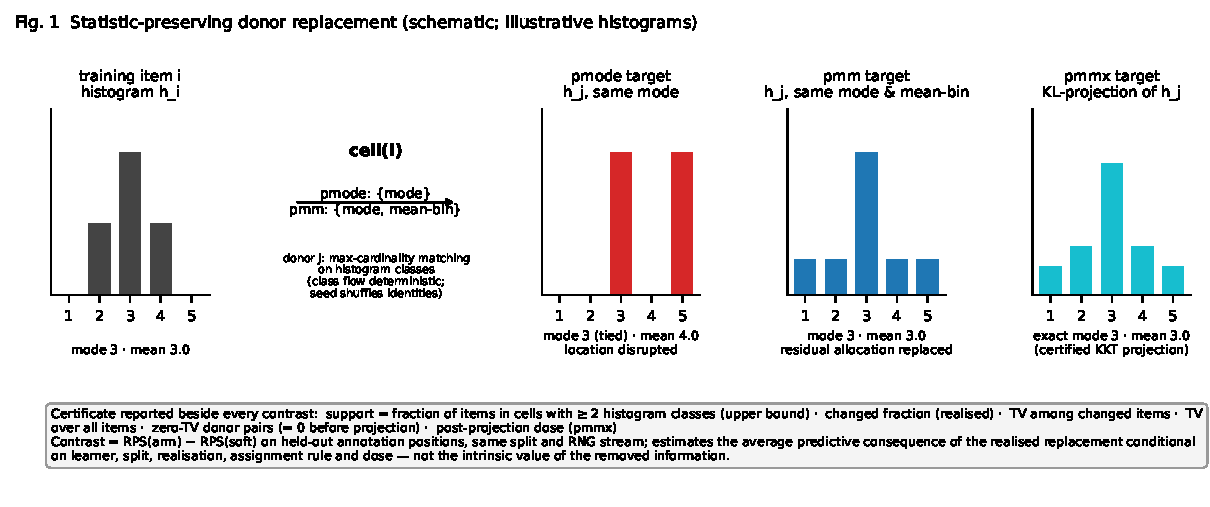
\includegraphics[width=0.9\textwidth]{../results/figures/fig1_schematic.pdf}
\caption{Statistic-preserving donor replacement (schematic; illustrative histograms). For a training item with histogram $h_i$, a donor histogram from another training item is assigned within a mode cell (pmode) or a mode-and-mean-bin cell (pmm); the exact variant (pmmx) KL-projects the donor to the recipient's mode and mean. The certificate reported beside every contrast lists support, realised changed fraction, TV among changed items, TV over all items and the zero-TV donor-pair count (0 before projection). Constrained donor construction does not imply statistical independence between original and replacement targets; the class-level assignment flow is deterministic given class sizes and the seed shuffles item identities within it.}\label{fig:schematic}\end{figure*}
\begin{figure*}[t]\centering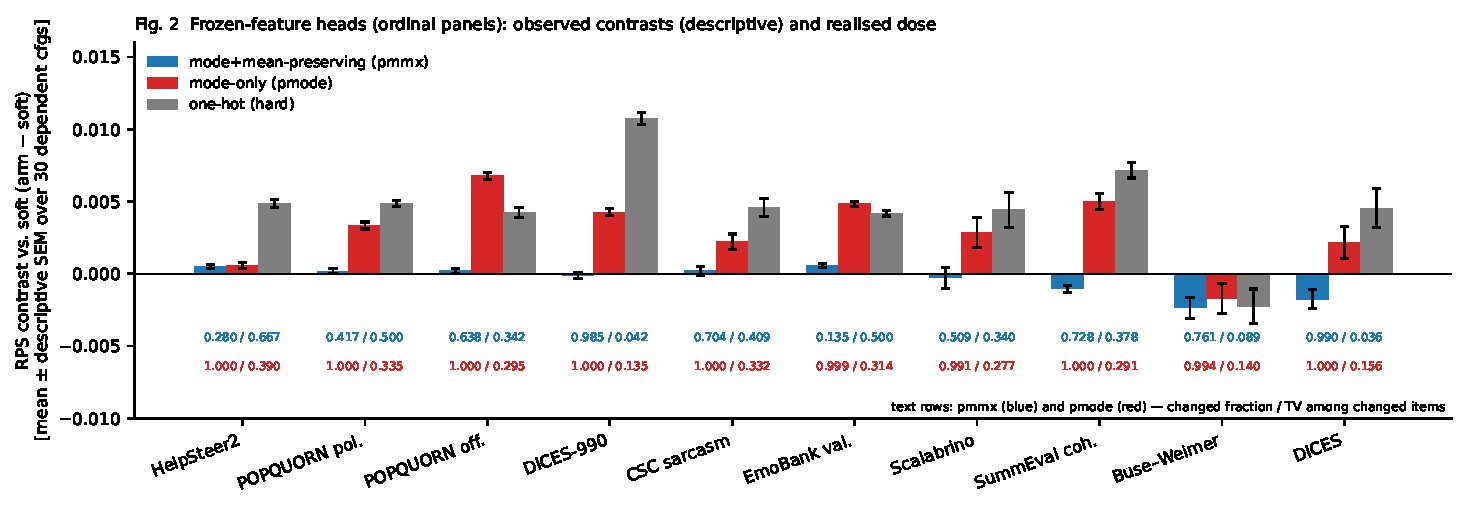
\includegraphics[width=0.95\textwidth]{../results/figures/fig2_heads_contrasts.pdf}
\caption{Frozen-feature heads: observed RPS contrasts (arm $-$ soft) for exact mode-and-mean-preserving replacement (pmmx), mode-only replacement (pmode) and one-hot targets (hard) on ten ordinal panels. Bars are means and error bars descriptive SEMs over 30 dependent configurations (5 RNG streams $\times$ 3 item splits $\times$ 2 annotation-position splits); they are not inferential intervals, and the figure supports only descriptive average contrasts across the tested panels, splits and training realisations. Text under each panel gives the realised post-projection changed fraction and TV among changed items for pmmx (blue) and pmode (red).}\label{fig:heads}\end{figure*}
\begin{figure*}[t]\centering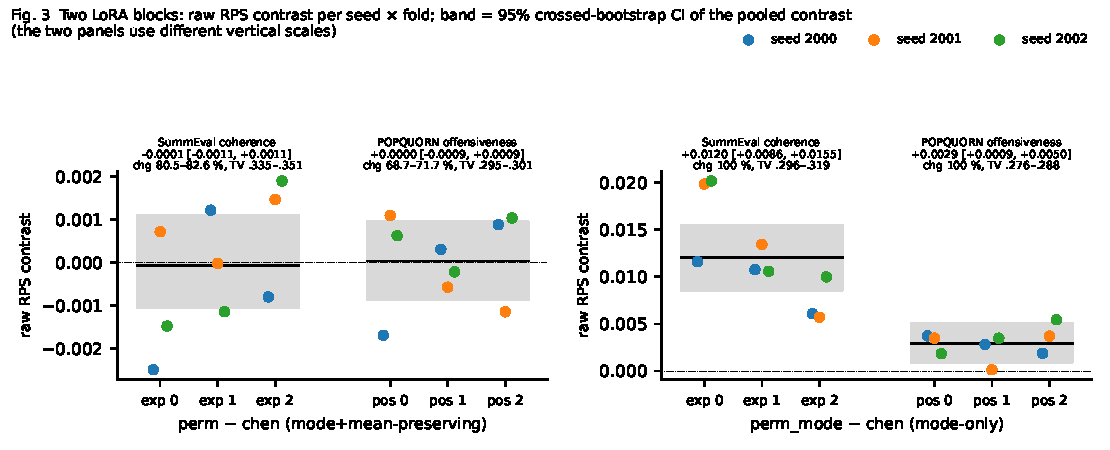
\includegraphics[width=0.85\textwidth]{../results/figures/fig3_summeval_block.pdf}
\caption{SummEval coherence LoRA replication block. Points are the nine seed-by-expert-fold raw RPS contrasts (three optimizer seeds, each paired with one item-assignment seed; seed-wise horizontal jitter). The band is a crossed-bootstrap 95\% interval for their pooled contrast, resampling optimizer--assignment clusters and test documents; it is not a range of cell effects. Left: mode-and-mean-preserving replacement (perm $-$ chen; 80.5--82.6\% of targets changed, TV among changed 0.335--0.351). Right: mode-only replacement (perm\_mode $-$ chen; 100\% changed, TV 0.296--0.319). Panels use different vertical scales.}\label{fig:summeval}\end{figure*}
\begin{figure*}[t]\centering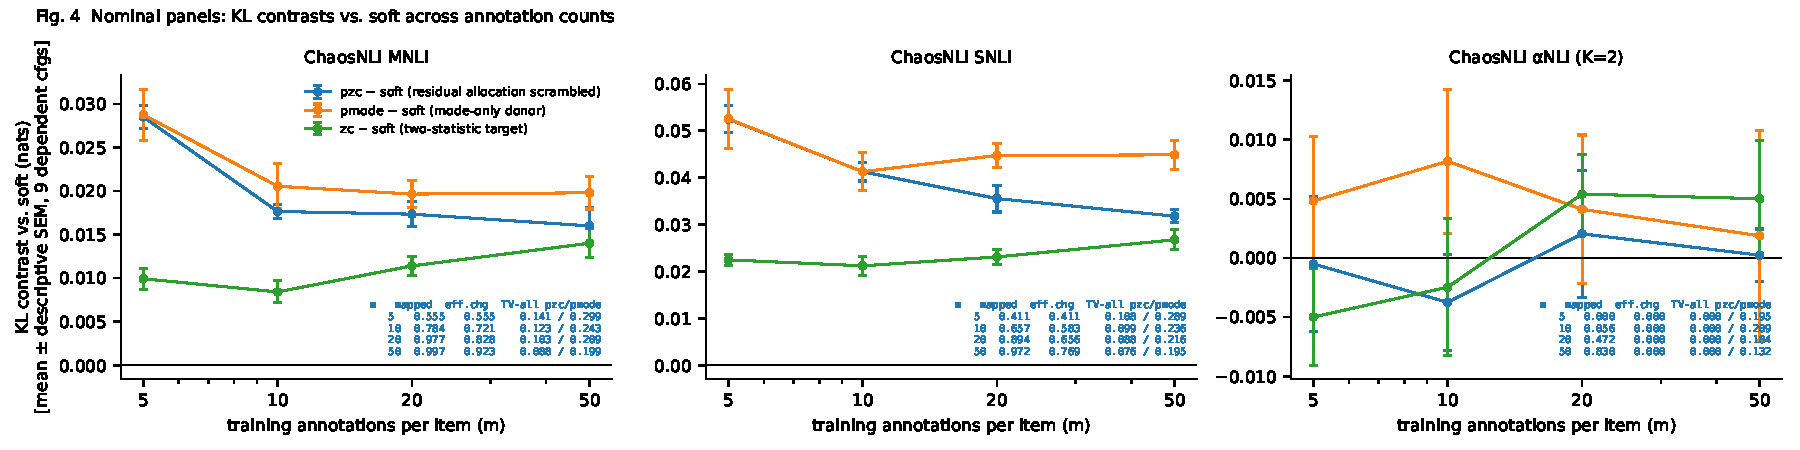
\includegraphics[width=0.95\textwidth]{../results/figures/fig4_chaosnli.pdf}
\caption{ChaosNLI nominal panels (MNLI, SNLI, $\alpha$NLI; on $\alpha$NLI the pzc intervention has zero final dose by construction): mean test KL to a fixed 50-annotation reference panel, contrasts vs.\ training on the $m$-annotation histogram, for residual-allocation scrambling with modal class and mass preserved (pzc), mode-only donor replacement (pmode) and the two-statistic target (zc); means and descriptive SEMs over nine dependent configurations. Blue text: mapped fraction, an effective-change sensitivity (TV $>10^{-6}$) and the final TV over all items. A descriptive sensitivity to nested annotation-subsample size, not a causal annotation-count curve.}\label{fig:nominal}\end{figure*}
